\documentclass[12pt,letterpaper]{article}
\usepackage[utf8]{inputenc}
\usepackage[spanish]{babel}
\usepackage{graphicx}
\usepackage[left=2cm,right=2cm,top=2cm,bottom=2cm]{geometry}
\usepackage{graphicx} % figuras
% \usepackage{subfigure} % subfiguras
\usepackage{float} % para usar [H]
\usepackage{amsmath}
%\usepackage{txfonts}
\usepackage{stackrel} 
\usepackage{multirow}
\usepackage{enumerate} % enumerados
\renewcommand{\labelitemi}{$-$}
\renewcommand{\labelitemii}{$\cdot$}
% \author{}
% \title{Caratula}
\begin{document}

% Fancy Header and Footer
% \usepackage{fancyhdr}
% \pagestyle{fancy}
% \cfoot{}
% \rfoot{\thepage}
%

% \usepackage[hidelinks]{hyperref} % CREA HYPERVINCULOS EN INDICE

% \author{}
\title{Caratula}

\begin{titlepage}
\begin{center}
\large{UNIVERSIDAD PRIVADA-DE-TACNA}\\
\vspace*{-0.025in}
\begin{figure}[htb]
\begin{center}

\includegraphics[width=8cm]{./Imagenes/logo}
\end{center}
\end{figure}
\vspace*{0.15in}
INGENIERIA DE SISTEMAS  \\

\vspace*{0.5in}
\begin{large}
TITULO:\\
\end{large}

\vspace*{0.1in}
\begin{Large}
\textbf{INFORME DE LABORATORIO Nº 07} \\
\end{Large}

\vspace*{0.3in}
\begin{Large}
\textbf{CURSO:} \\
\end{Large}

\vspace*{0.1in}
\begin{large}
BASE DE DATOS II\\
\end{large}

\vspace*{0.3in}
\begin{Large}
\textbf{DOCENTE(ING):} \\
\end{Large}

\vspace*{0.1in}
\begin{large}
 Patrick Cuadros Quiroga\\
\end{large}

\vspace*{0.2in}
\vspace*{0.1in}
\begin{large}
Alumno: \\
\begin{flushleft}
Acosta Ortiz, Orlando Antonio                  \hfill	(2015052775) \\
\end{flushleft}
\end{large}
\end{center}

\end{titlepage}


\tableofcontents % INDICE
\thispagestyle{empty} % INDICE SIN NUMERO
\newpage
\setcounter{page}{1} % REINICIAR CONTADOR DE PAGINAS DESPUES DEL INDICE

\section{INFORMACIÓN GENERAL} 

\begin{itemize}
\subsection{Objetivos:}

	 \item Aprender y utilizar una importante herramienta como Azure Data Studio para la Monitorización de Base de Datos mediante Auditoría.
\subsection{Requerimientos}


	
    Para el desarrollo de esta práctica se requerirá de los siguientes        	  conocimientos básicos:
	\item Conocimientos básicos de administración de base de datos 	  			 Microsoft SQL Server.
	\item Conocimientos básicos de SQL.\\\\
	
	\item Tener Azure Data Studio Instalado.\\
	
	\begin{figure}[htb]
	\begin{center}
	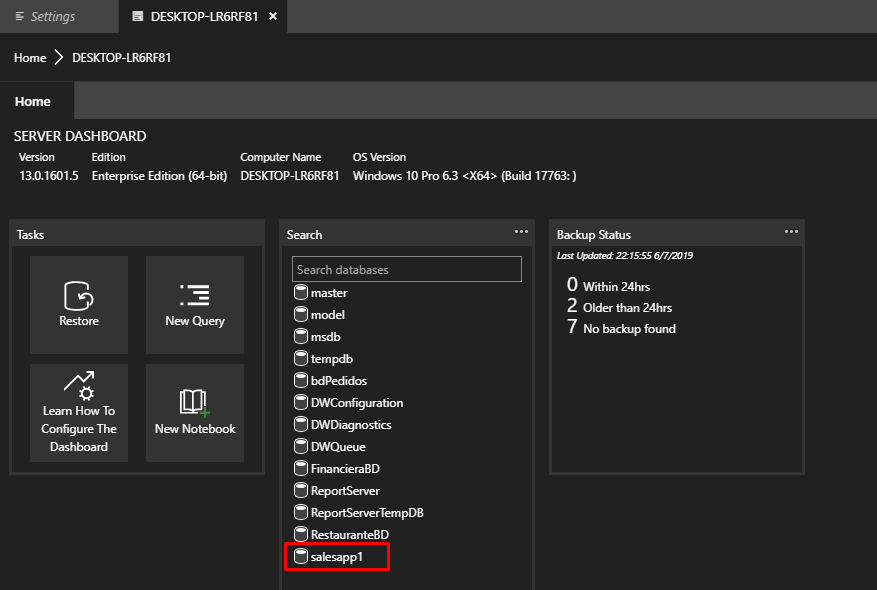
\includegraphics[width=15cm]{./Imagenes/audit0}
	\end{center}
	\end{figure}


\end{itemize}
\include{Secciones/Actividad02}
\section{Monitorización de Base de Datos mediante Auditoría} 

\begin{itemize}
\subsection{Aplicando auditorias}
	
	\item Paso 1: Crear una auditoría del servidor con las siguientes propiedades
	
	\begin{figure}[htb]
	\begin{center}
	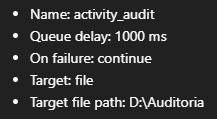
\includegraphics[width=9cm]{./Imagenes/audit1}
	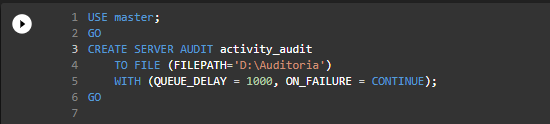
\includegraphics[width=9cm]{./Imagenes/audit2}
	\end{center}
	\end{figure}
	
	\item Paso 2: Activar la auditoria del servidor creada.

	\begin{figure}[htb]
	\begin{center}
	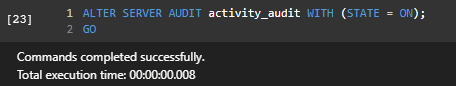
\includegraphics[width=9cm]{./Imagenes/audit3}
	\end{center}
	\end{figure}

	\item Paso 3: Crear una especificación de auditoría del servidor con las siguientes propiedades. \\\\
	\begin{figure}[htb]
	\begin{center}
	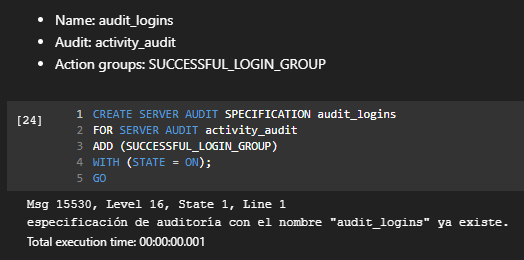
\includegraphics[width=9cm]{./Imagenes/audit4}
	\end{center}
	\end{figure}
	
	\item Paso 4: Activar la especificación de auditoria del servidor creada.\\\\\\\\
	\begin{figure}[htb]
	\begin{center}
	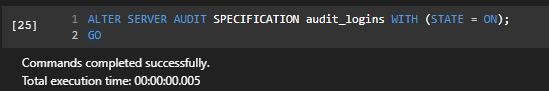
\includegraphics[width=9cm]{./Imagenes/audit5}
	\end{center}
	\end{figure}

	\item Paso 5:  Crear una especificación de auditoría de base de datos en la base de datos salesapp1 con las siguientes propiedades:
	\begin{figure}[htb]
	\begin{center}
	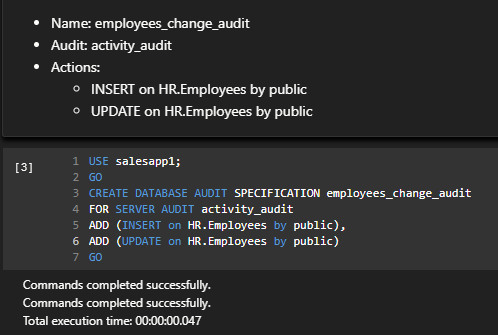
\includegraphics[width=9cm]{./Imagenes/audit6}
	\end{center}
	\end{figure}

	\item Paso 6: Activar la especificación de auditoría de base de datos creada.
	\begin{figure}[htb]
	\begin{center}
	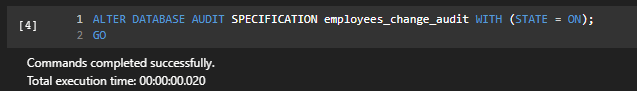
\includegraphics[width=9cm]{./Imagenes/audit7}
	\end{center}
	\end{figure}

	\item Paso 7: Ejecutar el siguiente código \\\\\\\\\\\\
	\begin{figure}[htb]
	\begin{center}
	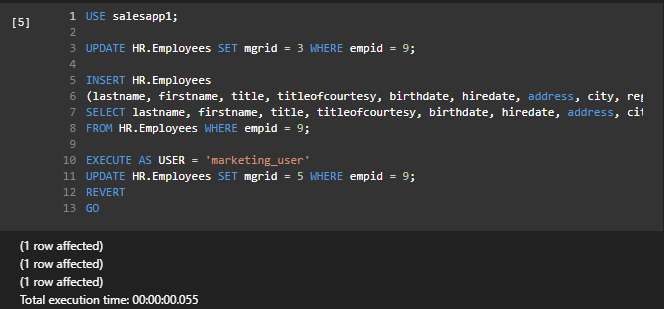
\includegraphics[width=9cm]{./Imagenes/audit8}
	\end{center}
	\end{figure}

	\item Paso 8: Escribir una consulta utilizando la función de sistema sys.fngetauditfile para devolver todos los datos de auditoría desde los archivos . 			 Filtrar los datos para que solo la actividad relacionada a la sesión actual sea visualizada. \\\\\\\\\\\\
	\begin{figure}[htb]
	\begin{center}
	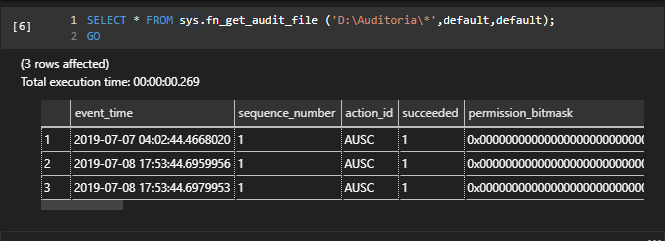
\includegraphics[width=9cm]{./Imagenes/audit9}
	\end{center}
	\end{figure}

	\item Paso 9 : Desahbilitar la auditoría de servidor activityaudit. \\\\\\\\\\\\
	\begin{figure}[htb]
	\begin{center}
	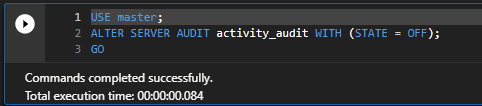
\includegraphics[width=9cm]{./Imagenes/audit10}
	\end{center}
	\end{figure}


\end{itemize}
\include{Secciones/Actividad04}
\section{CONCLUSIONES} 

\begin{itemize}
	\item Azure Data Studio nos permite administrar bases de datos SQL , nos facilita las consultas mucho mejor que el Software de Microsoft SSMS y en este caso nos permite monitorizar bases de datos
	
	

\end{itemize}
\include{Secciones/Actividad06}
\include{Secciones/Actividad07}
\end{document}
